
\section{Deliverable 3: XOR problem}


\begin{solve}    

\begin{figure}[H]
    \centering
    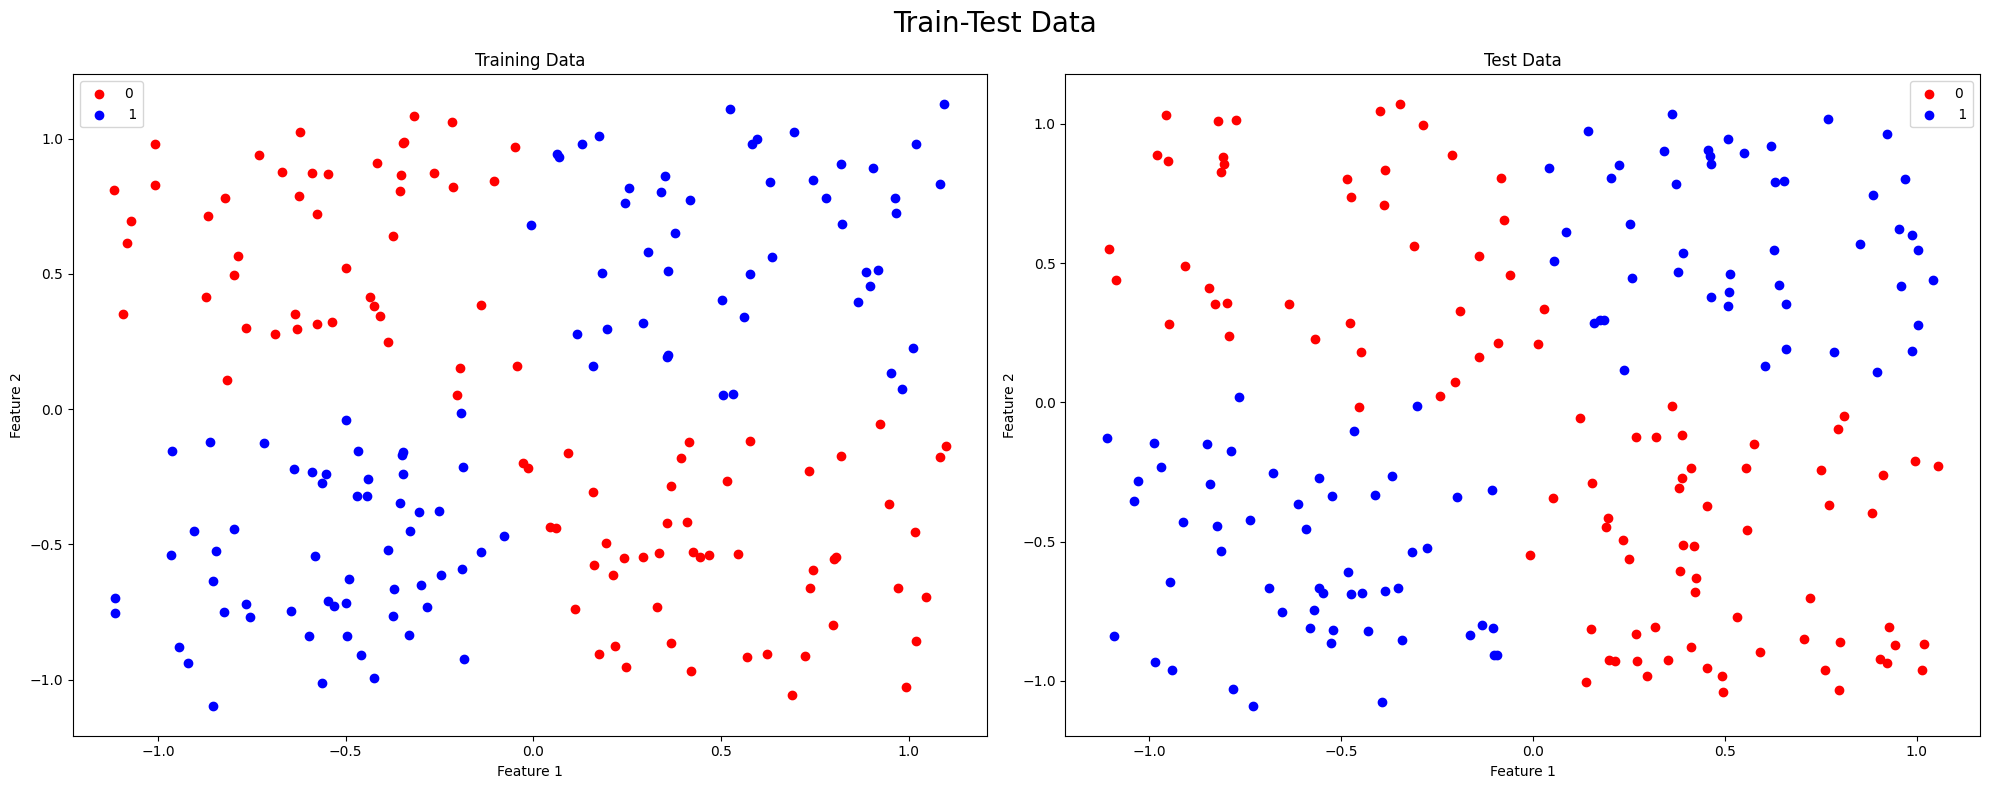
\includegraphics[width=0.7\textwidth]{plots/3_xor_dataset.png}
    \caption{XOR dataset (train, test set with 200 points each)}
\end{figure}

\begin{lstlisting}[language=python]
# one hot encoding the output to get the final output (dim 1 for prediction)

dim_in, dim_out = x_train.shape[1], 2
hidden_neuron_list = [4,16]
activation_list = ['ReLU', 'ReLU','Sigmoid']
opt_init = 'xavier'
opt_loss = L2Loss()
mlp = MLP(dim_in, dim_out, hidden_neuron_list, activation_list, opt_init)
opt_optim = Adam(mlp)
print(mlp.summary())
----------------------------------------

Model Summary
-------------
Layer 1: Linear - A Dim: 2, Output Dim: 4, Parameters: 12
Layer 2: ReLU
Layer 3: Linear - A Dim: 4, Output Dim: 16, Parameters: 80
Layer 4: ReLU
Layer 5: Linear - A Dim: 16, Output Dim: 2, Parameters: 34
Layer 6: Sigmoid
Total Parameters: 126
\end{lstlisting}

\begin{figure}[H]
    \centering
    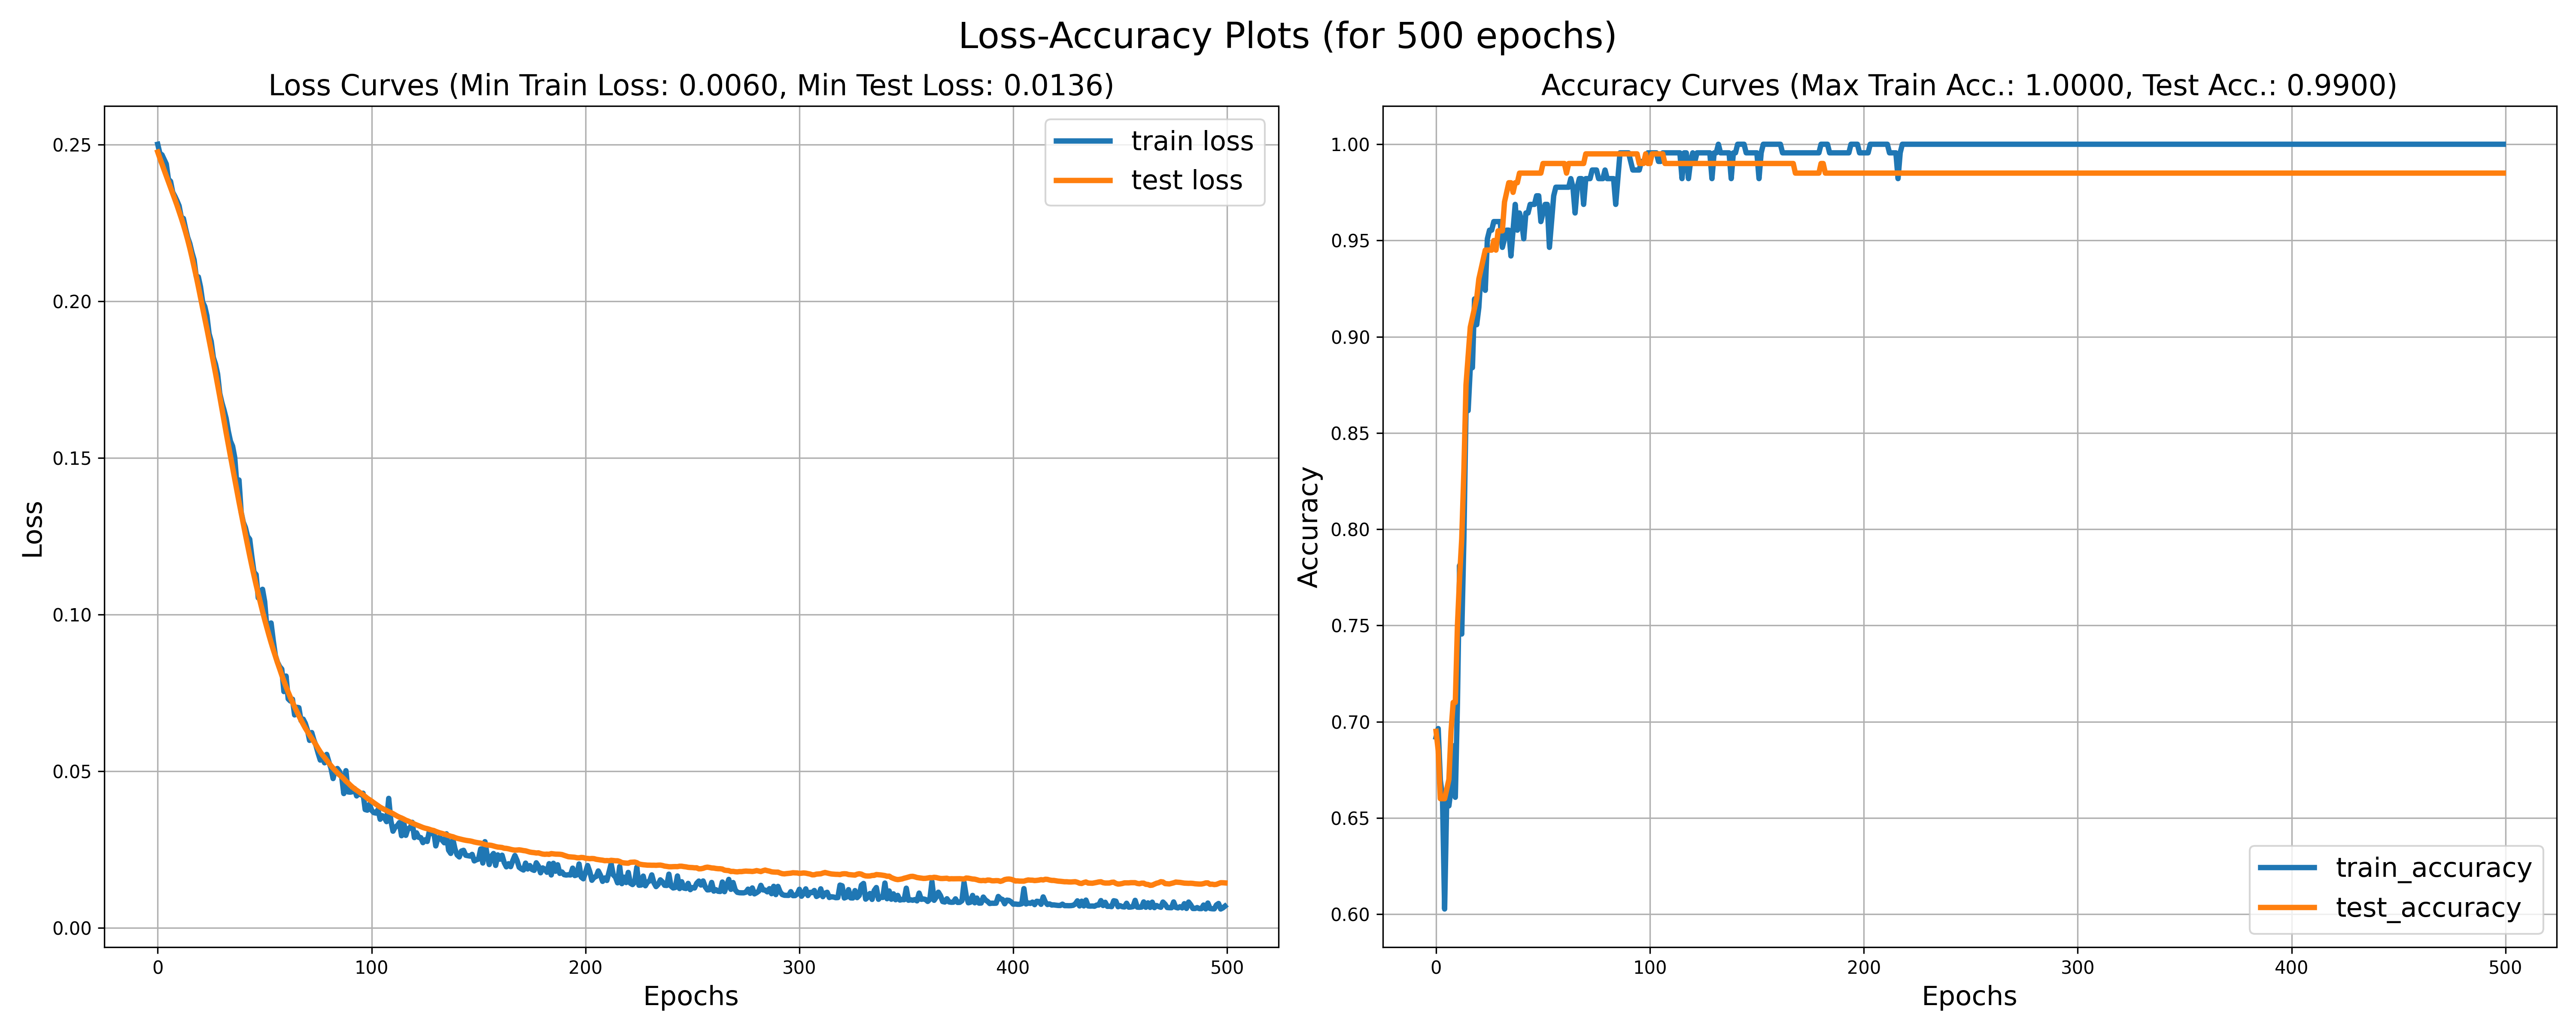
\includegraphics[width=0.9\textwidth]{plots/3_xor_adam_loss_acc.png}
    \caption{Loss and accuracy for XOR dataset (train, test set with 200 points each), Adam optimizer, 500 epochs, Cost function: L2Loss, Xaiver initialization}
\end{figure}

\begin{figure}[H]
    \centering
    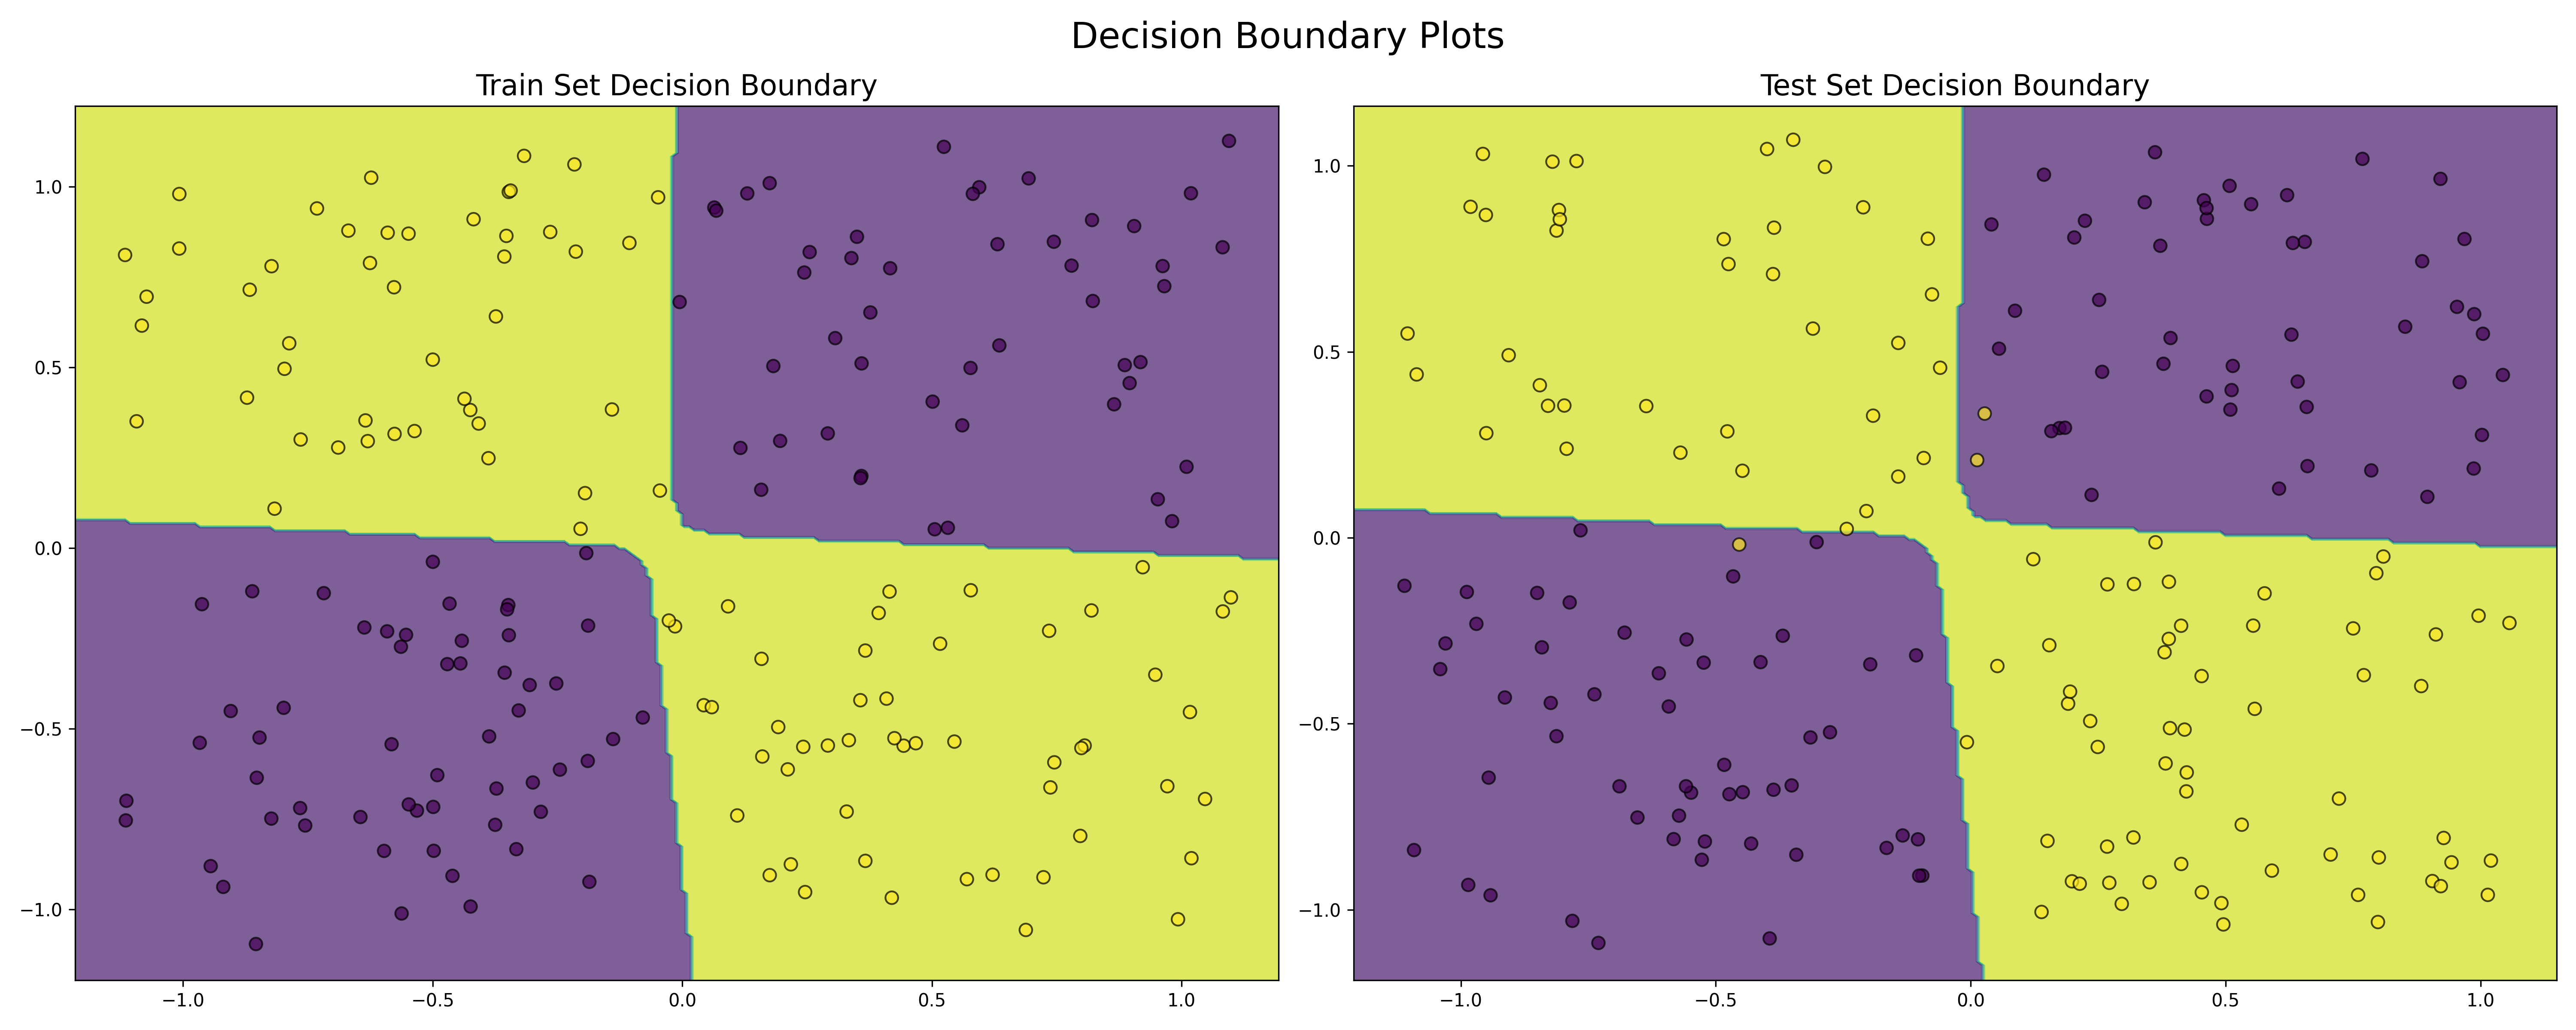
\includegraphics[width=0.8\textwidth]{plots/3_xor_adam_boundary.png}
    \caption{Decision boundary for XOR separable dataset (train, test set with 200 points each)}
\end{figure}

\end{solve}
